%!TEX root = ../thesis.tex

\section{Discussion}
\label{sec:discussion}

% TODO: Say that our properties only restrict machine-mode
% TODO: Say that we meet Alastair's requirements
% TODO: \glspl{ifc}
In section \ref{sec:checking}, a set of IFC properties based on the work in \cite{Ferraiuolo17} has been introduced; we will refer to these properties as the set $ P $.
These properties were model checked in the previous section \ref{sec:results}, the result of which was a set of rules $ R $.
What is the consequence of this?
The formal achievement of this thesis can be summarized as follows:
\begin{quote}
    It can be guaranteed that programs running on the MINRV8 architecture, e.g. \glspl{os}, are \textit{secure} (in the sense of not violating the IFC properties $ P $) if they obey to the rules $ R $.
\end{quote}
But what does \enquote{secure} mean here besides not violating $ P $?
What is the \textit{actual} sense of security that can be guaranteed?

Nothing definite can be said in answer to this question.
However, the canaries these properties have been tested against in section \ref{sec:canaries}, exemplify the class of vulnerabilities that are covered by these properties.

Assessing the results of the approach to formally verify higher level properties of the MINRV8 architecture shall be subject of this section.
We will cover four aspects of our work:
\begin{itemize}
    \item Scope, i.e. what are the limits of our results,
    \item Generalizability, i.e. how the proposed approach to verifying \glspl{isa} could be applied in other scenarios,
    \item Trustworthiness, i.e. whether our results are sound, and
    \item General observations.
\end{itemize}

\subsection{Scope}
\label{sec:scope}

\subsubsection{Architecture}

MINRV8 is meant to be a reasonable abstraction of a real-world \gls{riscv} architecture from a security standpoint.
However, up to this point nothing has been said about the limits of this abstraction.
With every abstraction, there is a small chance that it perfectly matches the concept that has been abstracted in regard to the purpose of the abstraction but in most cases, some corners are cut.
In this section, we will reflect on the limits of the MINRV8 architecture and its implementation.

% TODO: mention that other fields are well modelled
% TODO: mention that we actually don't need all computational instructions
% TODO: mention performance hit of dynamic memory regions

In summary, the MINRV8 architecture knows three groups of instructions (cf. table \ref{tbl:min-arch-instrs}):
\begin{itemize}
    \item Computational instructions such as \minrv{Mov}, \minrv{And}, \minrv{Add}, etc.
    \item Memory instructions \minrv{Load} and \minrv{Store}
    \item System instructions \minrv{Ecall}, \minrv{Mret}, \minrv{Csrrs}, \minrv{Csrrc}
\end{itemize}

A reader, experienced in the field of microcontrollers or computer-architecture in general might wonder why our model does not include:
\begin{enumerate}
    \item Executable memory and a \gls{pc}
    \item Jump or branch instructions
\end{enumerate}

The reason for both of these points lies in the implementation of the model.
In the introduction of the MINRV8 architecture in section \ref{sec:minrv8} we mentioned that the idea of the architecture was tightly coupled to its implementation in \gls{nuxmv}.
The design of the model had to answer the question: How can a stream of instructions be implemented?
nuXmv allows to think of the following options:
\begin{enumerate}
    \item \label{itm:exmem-frozen}
    Use \smv{FROZENVAR}s to model executable memory - a \smv{FROZENVAR} (frozen variable) is something like a constant in other programming languages but without a fixed value.
    nuXmv chooses the value on the first simulation step but does not change it afterwards.
    This is more efficient than using a plain \smv{VAR} and constraining it to not change, e.g. \smv{TRANS x = next(x);}.
    \item \label{itm:exmem-var}
    Use \smv{VAR}s to model executable memory.
    In practice, this would mean that the memory of the implementation as described in section \ref{sec:model-implementation} would be much larger than the current 4 bytes.
    \item \label{itm:exmem-ivar}
    Finally, use \smv{IVAR}s to model the stream of instruction.
    This is the option we decided to go for as described in section \ref{sec:model-implementation}.
    Using input variables means that there is no model of executable memory.
    Instead, the input variables provided to the implementation model a stream of a fully decoded instruction on each transition of the simulated model.
    As such, the architecture does not need to worry \textit{where} these instructions come from.
\end{enumerate}

The decision towards using input variables as a model of the stream of instructions was made because of two reasons:
\begin{enumerate*}[label=\alph*)]
    \item in the prototyping phase of the model, it was quickly found out that using input variables led to significant boosts in performance, and
    \item using input variable simplified the implementation significantly.
\end{enumerate*}
Having used purely either frozen variables or variables would have increased the size of the state space to be traversed by \gls{nuxmv} and would have introduced the necessity to implement instruction decoding increasing the complexity of the transition relation.
Furthermore, it would not have allowed for unbounded model checking of the architecture since the size of programs to be taken into consideration would have been bounded by the size of executable memory.

Yet, using input variables also has some downsides.
First and foremost, using input variables means that it is pointless to model a \gls{pc} or anything address related like return addresses, a dedicated \gls{lr} or \glspl{csr} such as \gls{mtvec} as without a model of executable memory there is nothing addresses could point to.
Instead, instructions will simply magically appear on each cycle of the processor model.
This means that the simulation is inaccurate in this regard which in itself is not a problem.
The model is supposed to be an abstraction.
Since it was decided to use input variables over a model of the \gls{mtvec} register and a \gls{pc}, the question now arises how accurately the implementation of the MINRV8 architecture is capable to simulate real architectures.
In a nutshell, the use of input variables over (frozen) variables introduces a certain sense of non-determinism to the model of the MINRV8 architecture when it comes to handling interrupts and exceptions.

\begin{figure}
    \centering
    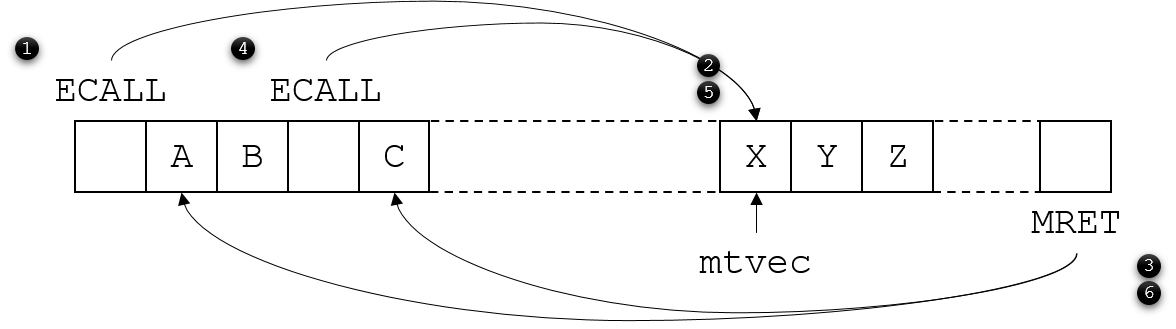
\includegraphics[width=0.7\textwidth]{figures/interrupt-flow.png}
    \caption{Program flow involving interrupts}
    \label{fig:interrupt-flow}
\end{figure}

Consider an example memory layout for the \gls{riscv} architecture as depicted in figure \ref{fig:interrupt-flow} where code is executed from left to right starting with an \minrv{Ecall} instruction.
Executing this instruction triggers a shift in control to machine-mode which jumps to address \minrv{X} pointed to by the \gls{mtvec} register.
Then, the instructions at addresses \minrv{X} to \minrv{Z} and subsequent ones are executed until finally, a \minrv{Mret} instruction is read an executed which triggers a jump to address \minrv{A}.
Two instructions later, another \minrv{Ecall} instruction is executed, etc.
We would expect the order of instructions to be executed to look like:

\begin{enumerate}
    \item First environment call: \lstinline[language=minrv8,mathescape=true]{Ecall, Load, Add, Store, $\dots$, Mret}
    \item Return: \lstinline[language=minrv8,mathescape=true]{Load, Mov}
    \item Second environment call: \lstinline[language=minrv8,mathescape=true]{Ecall, Load, Add, Store, $\dots$, Mret}
    \item Second return: \lstinline[language=minrv8,mathescape=true]{Slt, $\dots$}
\end{enumerate}
Where \minrv{Load, Add, Store} are the instructions located at addresses \minrv{X} to \minrv{Z} and \minrv{Load, Mov, Slt} the instructions located at addresses \minrv{A}, \minrv{B} and \minrv{C} respectively.

As input variables can not be constrained in \gls{nuxmv}, there is no way to model that the instructions being executed on a trap always are equal, i.e. a valid stream of instructions as a sequence of input variable valuations to the model might be:
\begin{enumerate}
    \item First environment call: \lstinline[language=minrv8,mathescape=true]{Ecall, Load, Add, Store, $\dots$, Mret}
    \item Return: \lstinline[language=minrv8,mathescape=true]{Load, Mov}
    \item Second environment call: \lstinline[language=minrv8,mathescape=true]{Ecall, And, Sra, $\dots$, Mret}
    \item Second return: \lstinline[language=minrv8,mathescape=true]{Slt, $\dots$}
\end{enumerate}

Such a stream of instructions is not realistic without some program modifying the code located at \gls{mtvec} and as such \enquote{shouldn't} be considered when checking the IFC properties.
One would expect to find the same code after an \minrv{Ecall} instruction being executed since in both cases, an architecture would jump to the respective interrupt handler.
However, there of course also exists a sequence of input variable valuations that exactly match a \enquote{real} stream of instructions where the instructions executed after an environment call coincide.

This illustrates one example for why the implementation of the MINRV8 \textit{abstracts} from real architectures.
In regard to program flow on traps, it can be expected that the model accurately comprises all expected streams of instructions but also includes many more one would naturally consider to be unrealistic.

The second concept, the abstract implementation of the MINRV8 architecture is missing are jump an branch instructions.
They are missing for the exact same reasons as described in the previous paragraphs.
Since the implementation does not support executable memory and as such does not support addresses, jumps and branches are pointless instructions.
This, however, does not turn out to be a fundamental problem.
In principle, jump and branch instructions in real systems are security relevant since they are used to perform function calls and returns and implement loops or conditional statements.
% TODO: \gls{rop}
In practice though, jumps and branches usually are security relevant since they are targeted by adversarial programs trying to manipulate jump addresses to launch ROP attacks.
ROP attacks are only effective because they jump to locations where critical code is located.
It does not matter whether the critical code is executed without the intervention of some malicious program or whether some malicious program tricks privileged code into executing said critical code - in practice, the former case simply occurs rarely.
The concept of jumps being influenced by some malicious program is, however, captured in approach: both properties \ref{itm:prop-mem-i} and \ref{itm:prop-csr-i}, i.e. the integrity of memory- and \gls{csr}- related instruction, ensure that certain instructions may not be influenced by user-mode.
There is no reason to assume that user-mode would control jumps and branches by fundamentally different flows of information than memory- and \gls{csr}-related instructions, i.e. jump related vulnerabilities are covered in principle.

Additionally, our implementation might not be able to model programs including jumps and branches but the set of programs considered by \gls{nuxmv} does include those where jumps have been linearized\footnote{%
    This is similar to function inlining supported by many compilers.
}.
Consider figure \ref{fig:jump-inlining} where in the upper half depicts an ordinary program, being executed from left to right and including jump instructions.
Jump linearization here means that for any such program there also exists another (potentially infinite) program where no jumps occur but the same instructions besides jumps are being executed.
The respective counterpart to the program in the upper half is depicted in the lower half of figure \ref{fig:jump-inlining}.
The sequence of states generated by the linearized programs is equal to the sequence of states of the non-linearized program modulo \gls{pc} values - which is not modelled in \gls{nuxmv} anyways.

\begin{figure}
    \centering
    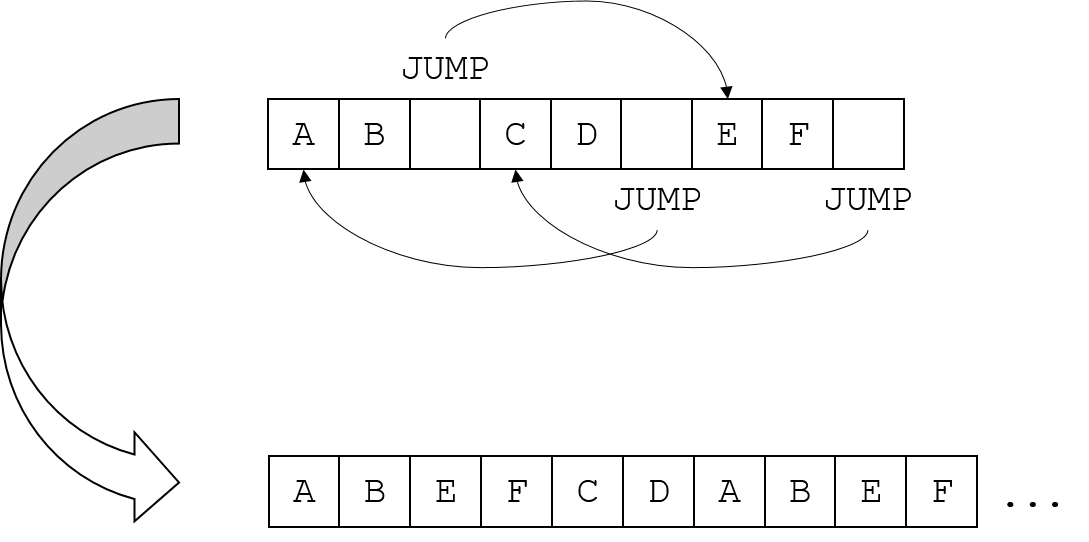
\includegraphics[width=0.7\textwidth]{figures/jump-free-programs.png}
    \caption{Jump linearization}
    \label{fig:jump-inlining}
\end{figure}

\paragraph{Summary}

Starting with the premise of this thesis, it was always clear that the MINRV8 architecture is a simplification.
This, though, is not a problem since by focusing on the very core, security related instructions allowed us to implement a tractable and small model in \gls{nuxmv}.
If one would add jump and branch instructions to the MINRV8 architecture, it'd be comparable to actual \gls{riscv} architectures.
From this point of view, it is not a problem to apply the results of the verification process, i.e. the set of assumptions, to the \gls{riscv} architecture.

The implementation of the MINRV8 architecture abstracted from real-world architectures in two main points:
\begin{enumerate}
    \item \gls{nuxmv} does not guarantee stable behavior on \minrv{Ecall} instructions; this introduces a sense of non-determinism for which there are more programs considered by \gls{nuxmv} than could actually be run on the MINRV8 architecture.
    This is not problematic because overabstracting the space of all programs $ P $ still leaves \gls{nuxmv} considering all programs in $ P $.
    \item The implementation does not support jump or branch instructions.
    This is not problematic because
    \begin{enumerate*}[label=\alph*)]
        \item flows of information relevant to jump and branch instructions are still covered by the integrity properties \ref{itm:prop-mem-i} and \ref{itm:prop-csr-i} and
        \item programs including jumps can be linearized; such programs \textit{are} considered by \gls{nuxmv}.
    \end{enumerate*}
\end{enumerate}

This leaves us with good reasons to assume that programs considered by \gls{nuxmv}, i.e. the set of programs quantified over when running proofs, is sufficiently close to the set of \enquote{real} programs of the MINRV8 architecture including jumps and branches.
% TODO: Future work?

\subsubsection{Assumptions}

\subsection{Generalizability}

\subsection{Trustworthiness}

\subsubsection{Model}

\subsubsection{Verification Process}
